\documentclass[UTF8,a4paper,10pt,fontset=none]{ctexart}
\usepackage[margin=20mm,headheight=15pt,footskip=12mm]{geometry}
\setCJKmainfont{Noto Serif CJK SC}
\setCJKsansfont{Noto Sans CJK SC}
\setCJKmonofont{Noto Sans Mono CJK SC}
\setmainfont{TeX Gyre Pagella}
\setsansfont{TeX Gyre Heros}
\setmonofont{DejaVu Sans Mono}[Scale=0.82]
\usepackage{amsmath,amssymb,graphicx,booktabs,tabularx,array,longtable,xcolor,fancyhdr,enumitem,listings,xurl,hyperref,lastpage}
\definecolor{brand}{HTML}{176B78}
\definecolor{ink}{HTML}{25333D}
\definecolor{pale}{HTML}{F0F5F6}
\hypersetup{colorlinks=true,linkcolor=brand,urlcolor=brand,pdfauthor={PulsarV},bookmarksnumbered=true}
\graphicspath{{../../images/}}
\ctexset{section={format=\Large\sffamily\bfseries\color{brand}},subsection={format=\large\sffamily\bfseries\color{ink}}}
\pagestyle{fancy}\fancyhf{}
\fancyhead[L]{\small\sffamily MOHISM VINS}
\fancyhead[R]{\small\sffamily\DocName}
\fancyfoot[L]{\small\sffamily\DocCode\enspace |\enspace Rev. 1.0}
\fancyfoot[R]{\small\thepage\ /\pageref*{LastPage}}
\renewcommand{\headrulewidth}{0.3pt}
\setcounter{tocdepth}{1}
\setlength{\parindent}{0pt}\setlength{\parskip}{6pt}
\renewcommand{\arraystretch}{1.38}
\setlist{nosep,leftmargin=1.6em,topsep=4pt}
\newcolumntype{Y}{>{\raggedright\arraybackslash}X}
\newcommand{\code}[1]{\nolinkurl{#1}}
\setlength{\emergencystretch}{2em}
\newcommand{\note}[1]{\par\smallskip\noindent\colorbox{pale}{\parbox{\dimexpr\linewidth-2\fboxsep}{#1}}\par\smallskip}
\lstset{basicstyle=\ttfamily\footnotesize,backgroundcolor=\color{pale},frame=none,breaklines=true,columns=fullflexible,keepspaces=true,showstringspaces=false,xleftmargin=6pt,xrightmargin=6pt,aboveskip=7pt,belowskip=7pt}
\newcommand{\cover}[2]{
\begin{titlepage}
{\sffamily\color{brand}\Large MOHISM\hfill\small TECHNICAL DOCUMENTATION}\par
\vspace{16mm}
{\sffamily\bfseries\fontsize{34}{42}\selectfont MOHISM VINS}\par
\vspace{3mm}{\sffamily\fontsize{24}{32}\selectfont\DocName}\par
\vspace{4mm}{\color{brand}\large 双目视觉惯性设备}\par
\vspace{10mm}
\includegraphics[width=\linewidth]{#1}\par
\vfill
\begin{tabularx}{\linewidth}{@{}lY@{}}\toprule
文档编号 & \DocCode\\
文档版本 & 1.0\quad /\quad 2026-10-30\\
固件基线 & 0.5.0，源码基线 \code{03d9960}\\
作者 & PulsarV\quad\href{mailto:zhijiatao@outlook.com}{zhijiatao@outlook.com}\\
内容 & #2\\\bottomrule
\end{tabularx}
\vspace{6mm}
{\footnotesize 原创硬件与文档采用 CC BY-NC-SA 4.0；软件许可按仓库 \code{LICENSING.md}。}
\end{titlepage}}

\newcommand{\DocName}{产品规格书}
\newcommand{\DocCode}{MV-SPEC-001}
\hypersetup{pdftitle={MOHISM VINS 产品规格书}}
\begin{document}
\cover{01_MoSense_Hero.png}{系统组成、接口、电气与机械设计、数据格式及软件功能}
\tableofcontents
\vspace{8mm}
\section*{文档范围}
本文对应仓库 0.5.0 固件、板级连接和 MoSense 外壳设计。参数表中的“请求频率”指固件配置值；输出频率由曝光、采集、算法和 USB 调度共同决定。渲染图用于识别结构与接口，尺寸以机械工程图为准。

系统由双目单色相机、六轴 IMU、板端计算单元、后备 RTC、SD 启动存储和 USB 接口组成。笔记本可同时接收左右图像、深度和里程计，并通过两个独立串口执行参数配置与调试。
\note{光学基线、镜头焦距、视场角、整机重量、工作温度等级和功耗限值未在本版定义。配置模板中的内外参不是产品光学规格。}
\newpage
\section{系统规格}
\par\noindent\begin{tabularx}{\linewidth}{@{}p{31mm}Y@{}}\toprule
项目 & 配置\\\midrule
成像 & 双路单色、全局快门，原生每路 1280$\times$800\\
图像输入 & 两路 MIPI 输入，原始灰度采集，RAW10 使用 16 位内存容器\\
惯性测量 & 三轴加速度与三轴角速度，SPI 数据接口、数据就绪中断\\
运行系统 & Linux 5.10.160，PREEMPT\_RT；Buildroot 2023.02.6\\
启动介质 & SD 卡；固定 ENV 分区布局\\
USB & USB 2.0 High Speed，Device 模式；两个 UVC 与两个 CDC ACM\\
后备时钟 & I²C 日历时钟，\code{/dev/rtc0}；有效时钟在启动时恢复系统 UTC\\
视觉惯性输出 & 位姿、速度、状态、重置计数；MAVLink common\\
配置与地图 & 参数原子保存；标定文件覆盖；地图保存、载入与重定位\\\bottomrule
\end{tabularx}\par

\subsection{图像与惯性参数}
\par\noindent\begin{tabularx}{\linewidth}{@{}p{35mm}Y@{}}\toprule
项目 & 固件设置\\\midrule
双目采集请求 & 15 / 30 / 60 / 120 fps；默认 120 fps\\
双目 UVC 请求 & 15 / 30 / 60 fps；默认 60 fps\\
稠密深度请求 & 15 / 30 / 60 / 120 Hz，不超过采集率；默认 30 Hz\\
深度 UVC 请求 & \code{min(USB_FPS, DEPTH_FPS)}；默认 30 fps\\
IMU 输出数据率 & 加速度、角速度均为标称 416 Hz\\
加速度量程与比例 & $\pm2g$；0.000061 $g$/LSB\\
角速度量程与比例 & $\pm250$ °/s；0.00875 °/s/LSB\\
IMU 时间戳 & 数据就绪 IRQ 入口的 CLOCK\_MONOTONIC，单位 ns\\\bottomrule
\end{tabularx}\par

\subsection{时钟与同步}
左右相机共用 FSIN，硬件 PWM 按采集配置生成触发脉冲。IMU INT1 独立报告数据就绪；算法使用标定时延与插值对齐图像和 IMU。当前驱动读取输出寄存器，未启用传感器 FIFO 和内部时间戳。共同 DEN 事件、门控与反馈路径属于独立的同步扩展设计。

RTC 记录日历时间，VIO 使用单调时钟。调整 RTC 或系统日期不改变 VIO 时间基准。RTC 的 INT 与 CLKOUT 未使用。
\newpage
\section{USB 与数据接口}
\par\noindent\begin{tabularx}{\linewidth}{@{}p{29mm}p{24mm}Y@{}}\toprule
功能 & 接口号 & 格式与用途\\\midrule
双目 UVC & 0 / 1 & 640$\times$200 YUYV，左右各 320$\times$200\\
深度 UVC & 2 / 3 & 320$\times$200 Z16，小端，毫米\\
MAVLink ACM & 4 / 5 & 板端 \code{/dev/ttyGS0}，参数、状态与里程计\\
调试 ACM & 6 / 7 & 板端 \code{/dev/ttyGS1}，日志、登录与 Shell\\\bottomrule
\end{tabularx}\par

同一复合设备共用一个 USB 地址与 VID/PID。Linux 开发标识为 \code{1d6b:0104}。主机的 \code{/dev/videoN} 和 \code{/dev/ttyACMN} 随连接顺序变化，应结合接口号、格式及设备路径识别。

\subsection{双目灰度与深度}
双目每帧 256000 字节，每行 1280 字节；左图占前 640 字节，右图占后 640 字节。像素按 \code{[gray,128]} 排列，色度固定。深度每帧 128000 字节，每行 640 字节，像素为无符号 16 位整数。深度 0 表示无效，软件接受数值范围为 100--65534 mm；该编码范围不定义有效测距范围。

标定关闭时输出原始双目预览；启用有效标定后输出校正图。深度只在实际计算完成后更新，可重复最近结果；200 ms 无新结果则清零。双目与深度独立调度，主机文件序号不用于曝光配对。

\subsection{带宽预算}
\par\noindent\begin{tabularx}{\linewidth}{@{}YYY@{}}\toprule
双目 / 深度请求 & 纯图像负载 & 用途\\\midrule
15 / 15 fps & 5.76 MB/s & 低负载配置\\
30 / 30 fps & 11.52 MB/s & 均衡配置\\
60 / 30 fps & 19.20 MB/s & 默认配置\\
60 / 60 fps & 23.04 MB/s & 接近端点负载上限\\\bottomrule
\end{tabularx}\par

双目端点每微帧最多 2048 字节，深度端点 1024 字节，合计理论负载上限 24.576 MB/s，另有 UVC 头等开销。原生双目 1280$\times$800 灰度在 60 fps 时约需 122.88 MB/s，常规 USB 输出使用降采样图像。

\subsection{调试启动阶段}
U-Boot 提供独立 CDC 控制台，标识为 \code{1d6b:0105}，倒计时 5 秒。进入 Linux 时 USB 重新枚举。BootROM、DDR 初始化和 SPL 日志通过 UART2 查看；UART 配置为 115200、8N1。
\newpage
\section{供电、结构与安装}
\par\noindent\begin{tabularx}{\linewidth}{@{}p{34mm}Y@{}}\toprule
项目 & 设计配置\\\midrule
外部连接 & USB Type-C；USB VBUS 5 V 输入\\
USB 电流声明 & 固件描述符声明 500 mA；使用符合主机端口供电能力的连接\\
内部电源域 & 系统 3.3 / 1.8 V，DDR 1.35 V，核心 0.9 V；相机 2.8 / 1.8 / 1.2 V\\
板卡参考尺寸 & 80$\times$30 mm；以机械装配参考板为准\\
镜头孔中心距 & 机械设计约 50 mm；光学平移使用双目标定结果\\
外壳 & CNC 铝合金，黑色表面涂层；前盖与背部散热壳分体\\
紧固 & 4 颗 M2.5$\times$14 沉头螺钉，配 4 颗 M2.5 六角螺母；壳体通孔，不攻丝\\
通孔 / 螺母槽 & 通孔 $\varnothing$2.90 mm；六角槽对边 5.20 mm，深 3.30 mm，详见加工公差\\
散热结构 & 9 条鳍片，间距 3.6 mm，名义厚 1.2 mm；中间 5 条长 78 mm，外侧 4 条长 62 mm\\
导热连接 & 名义 10$\times$10$\times$4 mm 导热垫，装配间隙约 3.47 mm\\\bottomrule
\end{tabularx}\par

\begin{center}
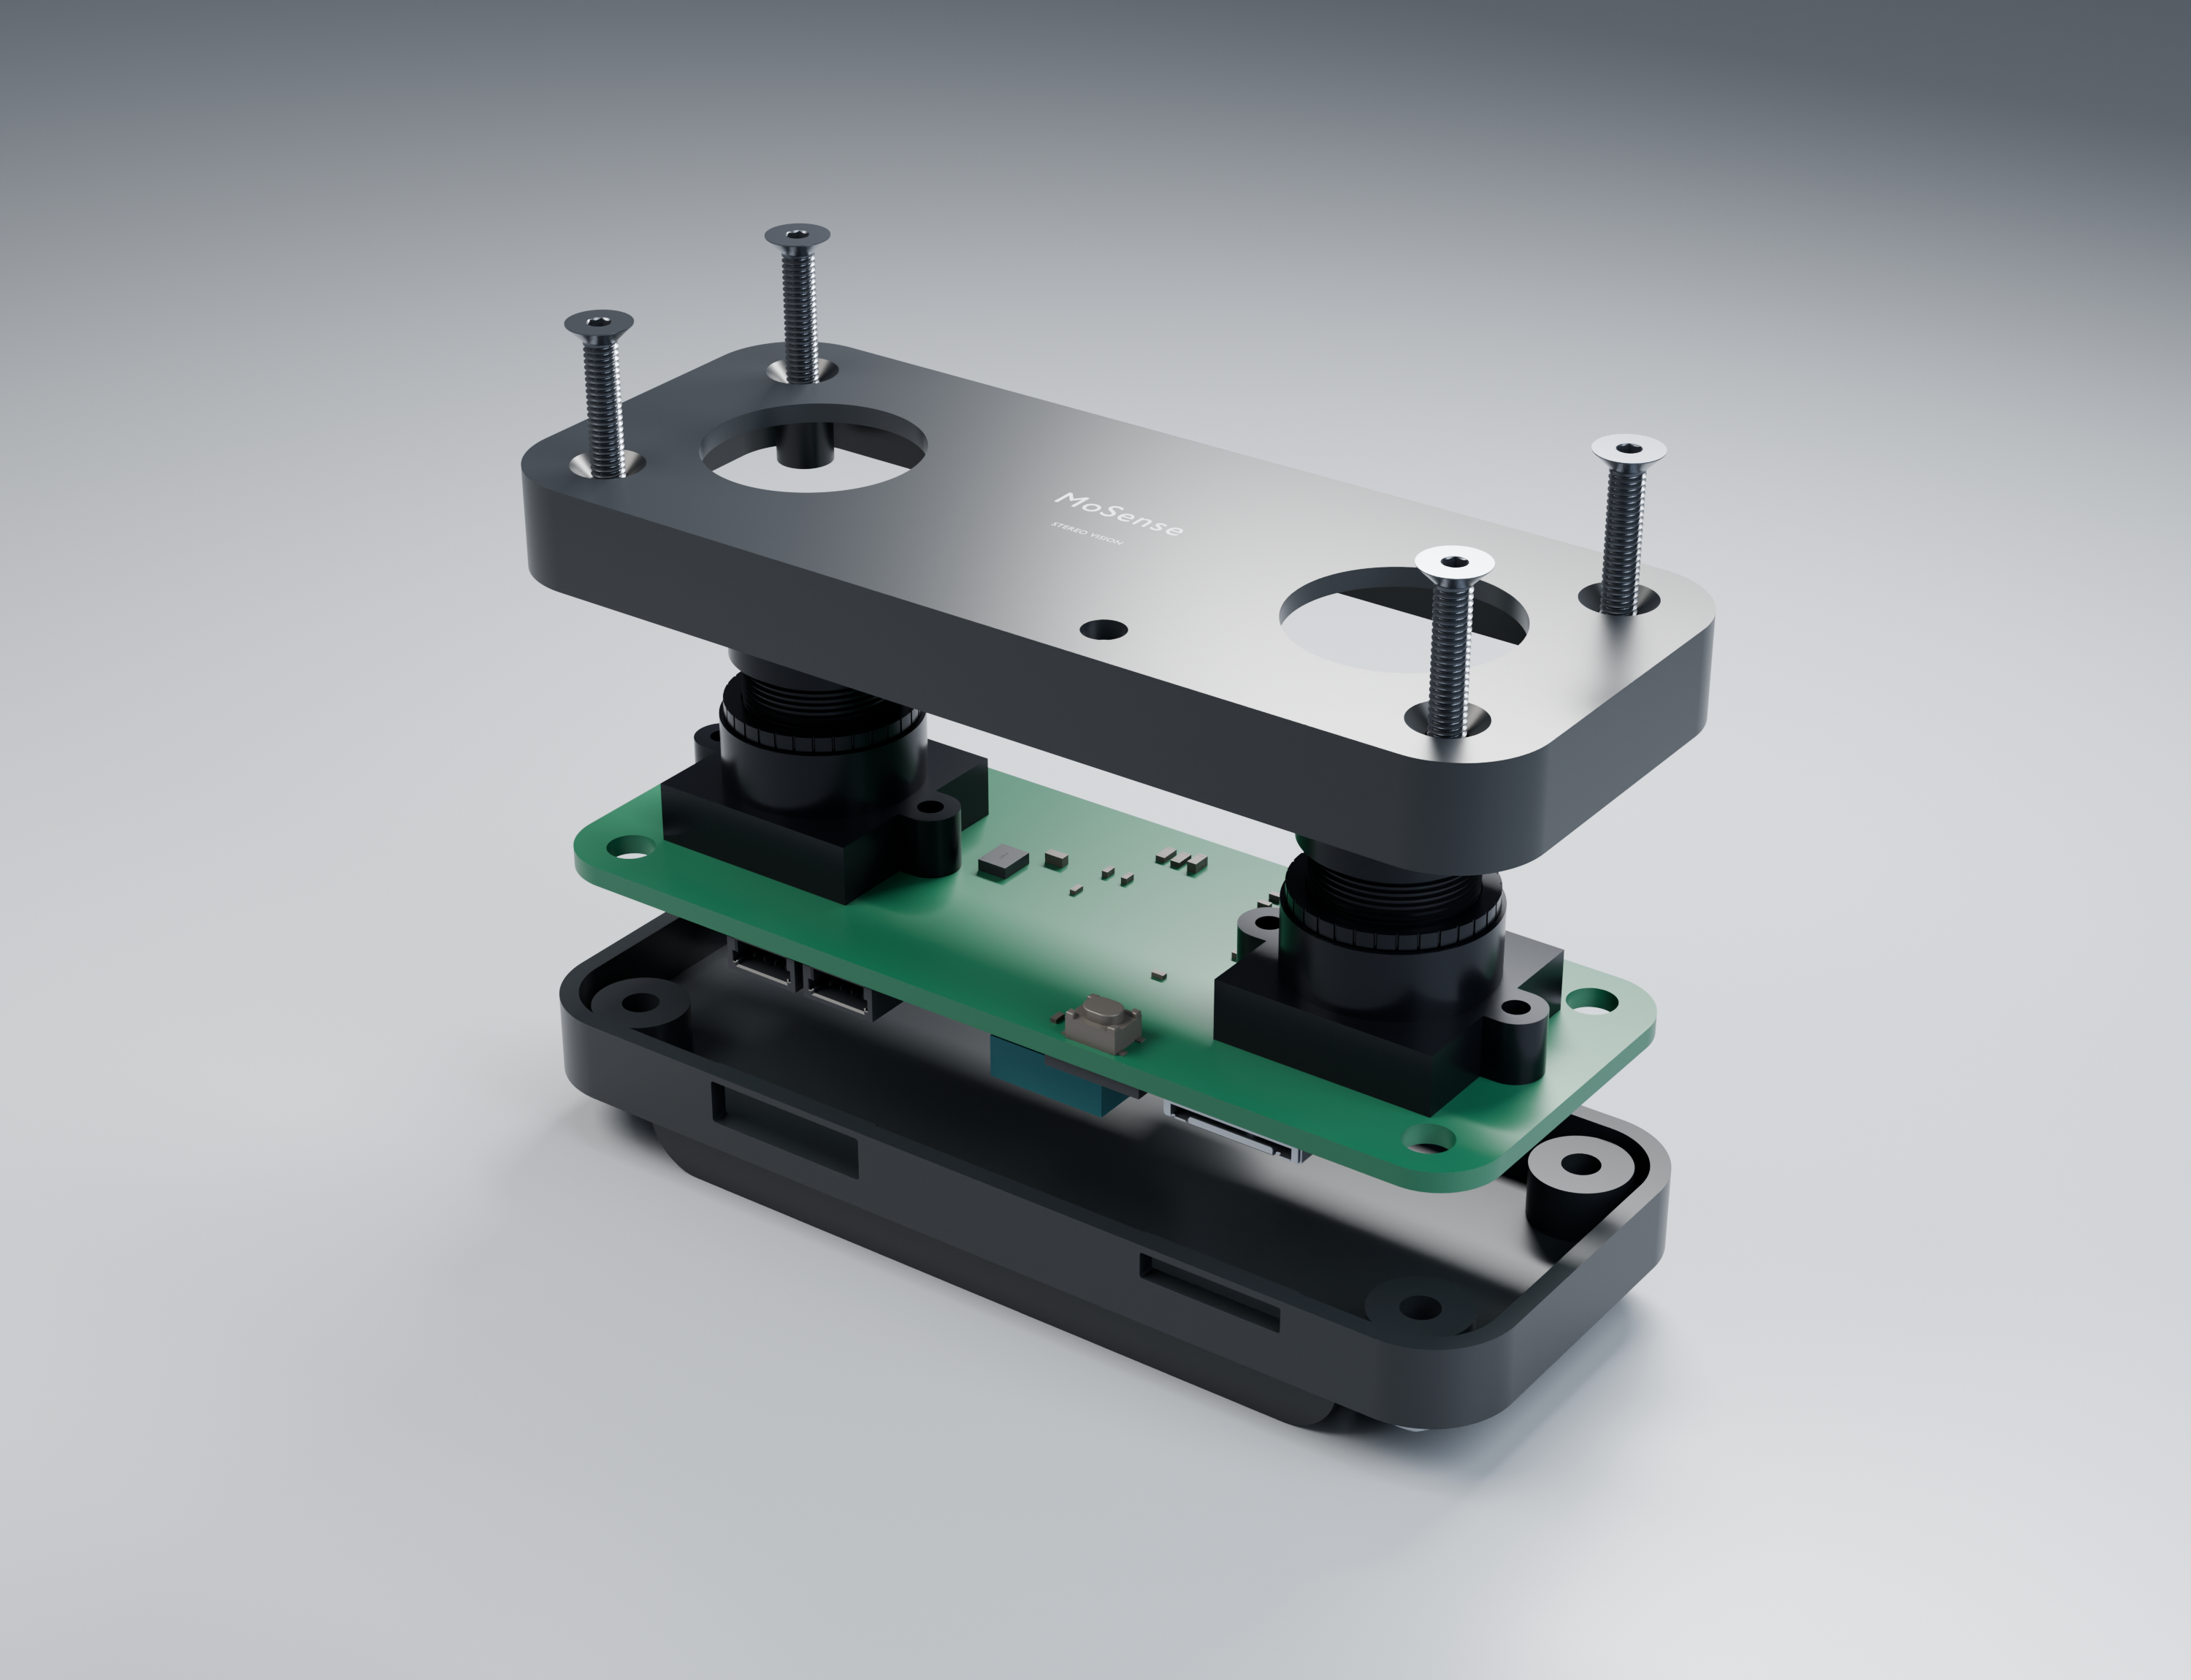
\includegraphics[width=.83\linewidth,height=65mm,keepaspectratio]{05_MoSense_Exploded.png}\\
{\small 前盖、板卡、背部散热壳与紧固件}
\end{center}

\subsection{安装约束}
镜头保持无遮挡，外壳散热鳍片留出空气通道；线缆固定在支架侧，减少插头载荷和图像振动。安装姿态变化后应核对机体坐标与 IMU 轴向标定。松动或调整镜头、相机板与壳体连接后，重新检查双目标定。

浮动螺母从后侧放入六角槽，前侧插入螺钉锁紧。螺母槽用于防转，不作过盈压入。螺母承压面、通孔与槽内表面遮蔽喷涂；详细尺寸链以机械加工文件为准。
\newpage
\section{算法、协议与配置}
\subsection{视觉惯性处理}
前端使用双向 LK 跟踪、空间补点与双目几何检查；后端使用 Ceres 紧耦合滑窗联合优化位姿、速度、偏置和特征逆深度。旧状态通过 Schur 边缘化保留信息。支持静止初始化及运动初始化、ORB 回环、四自由度位姿图和跨会话地图重定位。

默认滑窗 6 帧、最多 100 个特征、每次求解最多 8 次迭代，求解预算 40 ms，联合优化请求 30 Hz。在线外参和时间偏移估计默认关闭。地图默认保留 200 个关键帧，写入 userdata；原子保存同时需要旧文件和临时文件空间。

\subsection{MAVLink 参数}
系统号 1，组件号 197，参数类型 REAL32。默认参数如下：
\par\noindent\begin{tabularx}{\linewidth}{@{}p{36mm}p{15mm}Y@{}}\toprule
参数 & 默认 & 作用 / 范围\\\midrule
\code{VIO_ENABLE} & 1 & 0/1，关闭估计但保持预览\\
\code{SYNC_MAX_MS} & 2 & 0.1--20 ms，并受标定配置上限约束\\
\code{VIO_VALID} & 0 & 只读，有效估计状态\\
\code{FW_VERSION} & 500 & 只读，表示 0.5.0\\
\code{ACC_NOISE} & 0.1 & 0.001--10，m/s²/$\sqrt{\mathrm{Hz}}$\\
\code{GYRO_NOISE} & 0.01 & 0.00001--1，rad/s/$\sqrt{\mathrm{Hz}}$\\
\code{ACC_BIAS_RW} & 0.0001 & 0.000001--0.1，m/s²/$\sqrt{\mathrm{s}}$\\
\code{GYRO_BIAS_RW} & 0.00001 & 0.0000001--0.1，rad/s/$\sqrt{\mathrm{s}}$\\\bottomrule
\end{tabularx}\par

噪声默认值用于初始配置，应由传感器标定结果替换。参数保存到 \code{/userdata/mohism-params.yml}；标定保存到 \code{/userdata/calibration.yml}。

\subsection{位姿输出约定}
\code{ODOMETRY} 使用板端单调时钟微秒；父坐标 LOCAL\_FRD，子坐标 BODY\_FRD。位置在世界坐标中，速度在机体坐标中，四元数顺序为 $[w,x,y,z]$，描述 body 到 world 的旋转。协方差与角速度字段为 NaN，quality 为 $-1$。\code{reset_counter} 在恢复、重新启用或地图坐标修正时变化，接收端按段处理轨迹。
\newpage
\section{评估记录与交付文件}
\subsection{离线回放}
EuRoC MH\_01\_easy 包含 3682 对图像、36820 条 IMU 数据。处理分辨率 320$\times$200，优化请求 20 Hz，回环开启。结果按连续有效且重置计数相同的段分别作 SE(3) 对齐，不拟合尺度。
\par\noindent\begin{tabularx}{\linewidth}{@{}YY@{}}\toprule
指标 & 记录值\\\midrule
有效输出 & 3619 / 3682，98.29\%\\
匹配真值 & 3607 帧\\
重置或坐标修正计数变化 & 25 次\\
分段位置 ATE RMSE & 0.05988 m\\
分段位置 ATE P95 & 0.15406 m\\
1 秒平移 RPE RMSE & 0.05476 m\\
1 秒旋转 RPE RMSE & 0.63353°\\\bottomrule
\end{tabularx}\par

该结果描述分段离线轨迹，完整报告包含无效状态、逐段时长和未匹配帧。数据来源、SHA256 和结果保存在 \code{qualification/euroc-mh01-*.json}。

\subsection{交付目录}
\par\noindent\begin{tabularx}{\linewidth}{@{}p{60mm}Y@{}}\toprule
文件 & 内容\\\midrule
\code{out/artifacts/mohism-sd.img} & 完整 SD 卡镜像\\
\code{boot.img} / \code{uboot.img} & 内核与设备树 FIT / 启动固件\\
\code{rootfs.img} & 根文件系统\\
\code{mohism-vins} / \code{mohism_imu.ko} & 用户态算法 / IMU 内核模块\\
\code{mohism-vins-source.tar.gz} & 对应源码归档\\
\code{SHA256SUMS} & 文件校验值\\\bottomrule
\end{tabularx}\par

\subsection{资料索引与许可}
软件接口依据 \code{docs/protocol.md}、\code{docs/imu-driver.md}；性能依据 \code{docs/performance.md}；同步与 RTC 依据 \code{docs/hardware-sync.md} 和 \code{docs/hardware/rtc.md}。外壳依据 MoSense 参数化装配及加工公差文件。

原创硬件与本文档采用 CC BY-NC-SA 4.0，未经另行授权禁止商业使用。用户态软件采用 GPL-3.0，其他组件按各自许可。授权范围以仓库 \code{LICENSING.md} 为准。
\end{document}
